\documentclass{beamer}
\usetheme{Singapore}
\setbeamercovered{transparent}

\usepackage[english]{babel}
\usepackage[utf8]{inputenc}
\usepackage{times}
\usepackage[T1]{fontenc}
\usepackage{graphicx}
\usepackage{ragged2e}
\justifying

\title{Exploratory Data Analysis}
\date{\small MATH 252 Progress Presentation}
\institute{Kathmandu University \\ Department of Computational Mathematics}
\author{Aayush Shrestha \and Anmol Jha}

\subject{Exploratory Data Analysis}

\begin{document}
	
	\begin{frame}
		\titlepage
	\end{frame}
	
	\begin{frame}{Outline}
		\begin{enumerate}
			\item Introduction
			\item Objective
			\item Progressed Work
			\item Work to Complete
		\end{enumerate}
	\end{frame}
	
	\section{Introduction}
	\begin{frame}{Exploratory Data Analysis}
		Exploratory Data Analysis (EDA) is a method of analyzing data using statistical summaries and graphical representations.
		
		EDA is a critical step in any Data Analysis or Data Science project as it provides a better understanding of data set variables and their relationships, and what data can reveal beyond formal modeling or hypothesis testing tasks. It aids in determining how to best manipulate data sources to obtain the required answers, making it easier for data scientists to discover patterns, detect anomalies, determine test hypotheses, and validate assumptions.
	\end{frame}
	
	\begin{frame}{Dashboard}
		A dashboard is basically a GUI for Data Visualization. A dashboard is a good choice if you need to summarize and present a lot of information on a single window.
		
		A dashboard is one of the major tools for presenting data as it gives at-a-glance views of key performance indicators (KPI) relevant to a particular objective.
		
		A dashboard helps Data Analysts and Data Scientists perform many data-related tasks and also provides a visual aid for other stakeholders to understand data and make accurate data-based decisions.
	\end{frame}
	
	\section{Objective}
	\begin{frame}{Goals for the Project}
		\begin{itemize}
			\item Familiarity with data cleaning, feature extraction, and data conversion.
			
			\item Describing the data using statistical methods such as mean, median, standard deviation, correlation, and so on.
			
			\item Implementation of different plots in R.
			
			\item Implementation of a dashboard.
			
			\item Understanding and explaining the trends and outliers in the data based on the domain.
		\end{itemize}
	\end{frame}
	
	\section{Progressed Work}
	\begin{frame}{Initial View}
		\begin{figure}
			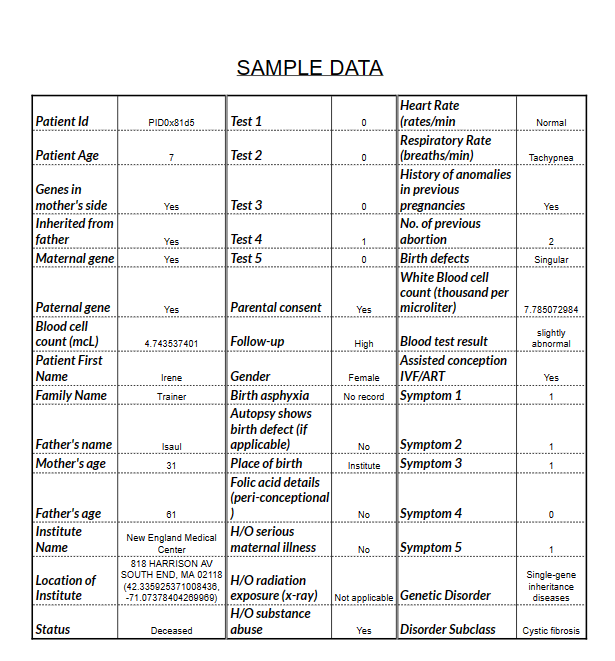
\includegraphics[width=0.65\textwidth, height=0.72\textheight]{sample.png}
			\caption{Sample raw data.}
		\end{figure}
	\end{frame}
	
	\begin{frame}{Initial Pre-processing}
		First of all, the data was changed from an \underline{xlsx} file to a \underline{csv} file, and the column names were modified to better suit programming. Also, all the rows with any NA values were removed.
		
		After completing all that, the dataset now contains 45 columns and 6706 observations.
	\end{frame}
	
	\begin{frame}{EDA Work}
		Exploring the columns and their types, the columns with data related to the patient but not the disorder were removed. Then, a statistical summary of the numeric columns was created, and the columns having no variance were also removed. We are left with 32 columns.
		
		Furthermore, based on graphical methods such as stacked bar graphs, box and whisker plots, and domain knowledge, a few more columns were disregarded based on their distribution and implication.
	\end{frame}
	
	\begin{frame}{Dashboard}
		% Content for the progressed dashboard work slide
	\end{frame}
	
	\section{Work to Complete}
	\begin{frame}{Remaining Work}
		\begin{itemize}
			\item Develop a better dashboard with more and better visual aids and information.
			
			\item Further reduce the dimensionality of the parameters based on more robust statistical and domain knowledge.
			
			\item Finally, create a properly processed dataset to be used for future classification projects.
		\end{itemize}
	\end{frame}
	
	
	\section*{}
	\begin{frame}
		\begin{center}
			{\Huge THANK YOU!} \newline \newline
		Please share if you have any queries.\newline
		We would like to show the code now.
		
	\end{center}
	\end{frame}
	
\end{document}
